\begin{frame}{El sonido}
  \begin{center}
    El \textbf{sonido} es una vibración en forma de onda.

    \bigskip
    \bigskip

    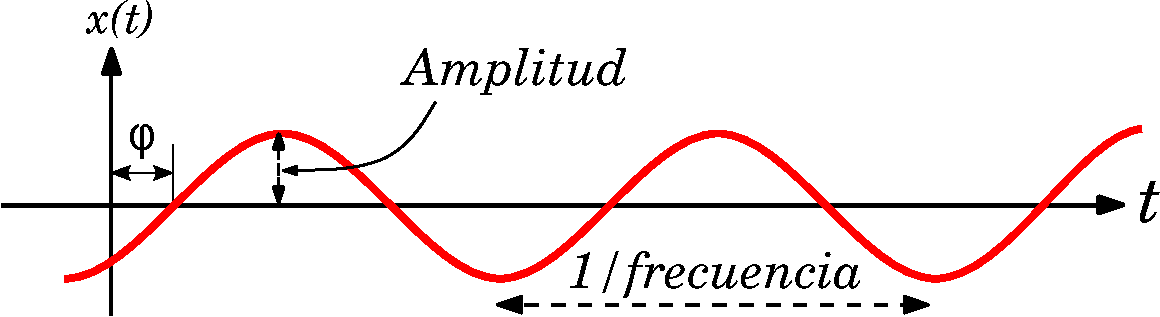
\includegraphics[width=0.8\textwidth]{imagenes/imagen_onda}

    \bigskip

    \begin{description}
    \item[Frecuencia] Oscilaciones por unidad de tiempo. Se relaciona con la
      altura de un sonido.
    \item[Amplitud] Energía que transporta la onda.
    \item[Fase] Desplazamiento respecto del origen.
    \end{description}
  \end{center}
\end{frame}

\begin{frame}{Descomposición de sonidos}
  Los sonidos no son ondas puras, se componen de \textbf{parciales}.

  \pause
  \bigskip
  
  La \textbf{frecuencia fundamental} es el menor de esos parciales.

  \pause
  \bigskip


\end{frame}


%%% Local Variables: 
%%% mode: latex
%%% TeX-master: "../presentacion"
%%% End: 
